\documentclass[11pt]{memoir}

\usepackage[top=1in, bottom=1.5in, left=1in, right=1in]{geometry}
\usepackage[notcite,notref,color]{showkeys}

\usepackage[pdftex,colorlinks=true,citecolor=blue,linkcolor=blue]{hyperref}
\usepackage{latexsym}
\usepackage{amsfonts}
\usepackage{amssymb}
\usepackage{amsmath}
\usepackage{url}
\usepackage{color}
\usepackage{graphicx}
\usepackage{epstopdf}
\DeclareGraphicsRule{.tif}{png}{.png}{`convert #1 `dirname #1`/`basename #1 .tif`.png}

% Define the listings environment
\usepackage{listings}
\usepackage{textcomp}
\definecolor{listinggray}{gray}{0.95}
\definecolor{lbcolor}{rgb}{0.9,0.9,0.9}
\lstset{
        numbers=left,
        numberstyle=\tiny,
        stepnumber=1,
        	backgroundcolor=\color{listinggray},
	tabsize=4,
	rulecolor=,
	language=C,
        basicstyle=\scriptsize,
        upquote=true,
        aboveskip={1.1\baselineskip},
        columns=fixed,
        showstringspaces=false,
        extendedchars=true,
        breaklines=true,
        prebreak = \raisebox{0ex}[0ex][0ex]{\ensuremath{\hookleftarrow}},
        frame=single,
        showtabs=false,
        showspaces=false,
        showstringspaces=false,
        identifierstyle=\ttfamily,
        keywordstyle=\bfseries\ttfamily\color[rgb]{0,0,1},
        commentstyle=\ttfamily\color[rgb]{0.1,0.6,0.2},
        stringstyle=\ttfamily\color[rgb]{1,0.1,0.3},
        linewidth=0.97\linewidth,
        xleftmargin=18pt,
}

% Define the frame environment
\usepackage{frame}
\definecolor{shadecolor}{rgb}{1,0.9,0.1}

%%%%%%%%%%%%%%%%%%%%%%%%%%%%%%
\newtheorem{theorem}{Theorem}[section]
\newtheorem{definition}[theorem]{Definition}
\newtheorem{algorithm}[theorem]{Algorithm}
\newtheorem{example}[theorem]{Example}
\newtheorem{remark}[theorem]{Remark}
%%%%%%%%%%%%%%%%%%%%%%%%%%%%%%


\title{\Huge FASP User Guide}

\author{FASP Developer Team}

\date{\vfill Version 1.3.6} % Activate to display a given date or no date

\begin{document}

\clearpage\maketitle
\thispagestyle{empty}

\newpage
\setcounter{page}{1}
\tableofcontents

%%%%%%%%%%%%%%%%%%%%%%%%%%%%%%
\chapter{Introduction}\label{ch:intro}
%%%%%%%%%%%%%%%%%%%%%%%%%%%%%%

%%%%%%%%%%%%%%%%%%%%%%%%%%%%%%
\section{What is FASP}\label{sec:goal}
%%%%%%%%%%%%%%%%%%%%%%%%%%%%%%

Over the last few decades, researchers have expended significant effort on developing efficient iterative methods for solving discretized partial differential equations (PDEs). Though these efforts have yielded many mathematically optimal solvers such as the multigrid method, the unfortunate reality is that multigrid methods have not been much used in practical applications. This marked gap between theory and practice is mainly due to the fragility of traditional multigrid (MG) methodology and the complexity of its implementation. We aim to develop techniques and the corresponding software that will narrow this gap, specifically by developing mathematically optimal solvers that are robust and easy to use in practice.

We believe that there is no one-size-for-all solution method for discrete linear systems from different applications. And, efficient iterative solvers can be constructed by taking the properties of partial differential equations (PDEs) and discretizations into account. In this project, we plan to construct a pool of discrete problems arising from systems of PDEs and efficient linear solvers for these problems. We mainly utilize the methodology of Auxiliary Space Preconditioning (ASP)~\cite{Xu.Xu.2010ff} to construct efficient linear solvers. Due to this reason, this software package is called ``Fast Auxiliary Space Preconditioning'' or FASP for short.

\subsection{Our goal}

The FASP project is not a traditional software project; instead, it is designed to support our effort to identify efficient algorithms and to build fast solvers for a set of PDE problems---FASP is designed for developing and testing new efficient solvers and preconditioners for discrete partial differential equations (PDEs) or systems of PDEs. The main components of the package are basic linear iterative methods, standard Krylov methods, geometric and algebraic multigrid methods, and incomplete factorization methods. Based on these standard techniques, we build efficient solvers, based on the framework of Auxiliary Space Preconditioning, for several complicated applications. For the moment, we have a few examples include the fluid dynamics, underground water simulation, the black oil model in reservoir simulation, and so on.

FASP contains the kernel part and several applications (ranging from fluid dynamics to reservoir simulation). The kernel part is open-source and licensed under GNU Lesser General Public License or LGPL. We tried and will continue to try to keep as many parts of the FASP project open to public as possible. However, some of the applications contain contributions from and owned partially by other parties. We only discuss the kernel functions (open to public) in this user's guide.

\begin{snugshade}\noindent
LICENSE: This software is free software distributed under the Lesser General Public
License or LGPL, version~3.0 or any later versions. This software distributed
in the hope that it will be useful, but WITHOUT ANY WARRANTY; without even
the implied warranty of MERCHANTABILITY or FITNESS FOR A PARTICULAR PURPOSE. See the GNU Lesser General Public License \url{http://www.gnu.org/licenses/} for more details.
\end{snugshade}

\subsection{Our strategy}

We organize the development of FASP package in a \emph{``Multilevel''} or \emph{``Capitalism''} way:

\begin{itemize}

\item Stage 1. Fine level stage (or free market stage)

\begin{enumerate}
\item[(1)] Collect problems and solvers. Allow similarities or even duplications, for example same solution algorithm, but different implementation. Keep all the record: problem description, solver code, test results, etc.
%
\item[(2)] Try to find a minimal set of standard or rules. And then we let the market to evolve freely. The idea is to allow the market to be FREE.
\end{enumerate}

\item Stage 2. Coarse level stage (or state capitalism stage)

\begin{enumerate}
\item[(1)] As FASP evolves, we might see, at certain time, that the market is out-of-control. This basically means the ``fine level solver'' or the ``free market'' is very successful and we should start to give more strict standard or regulation.
%
\item[(2)] Write a professional-level software package for a set of chosen algorithms for particular problems.
\end{enumerate}
\end{itemize}

%%%%%%%%%%%%%%%%%%%%%%%%%%%%%%
\section{What solvers you are going to get}\label{sec:idea}
%%%%%%%%%%%%%%%%%%%%%%%%%%%%%%

We are currently interested in the theory and numerical solution of many PDE problems. Currently, we are mainly working on solving the following PDEs and PDE systems (this is not a complete list and it is still expanding):
\begin{itemize}
\item Poisson equation
\item Reaction-diffusion equation
\item Linear elasticity
\item Brinkman equation
\item Biharmonic equation
\item Stokes and Navier-Stokes equations
\item Fluid-structure interaction
\item Oldryod-B and Johnson-Seglman equations
\item Darcy's flow
\item Black oil model and its generalizations
\item H(curl)/H(div) systems
\item Maxwell equation
\item MHD equation
\end{itemize}
%
We intend to design solution algorithms and their implementation for all these problems with different discretizations. We have done a few of them but not all of them are publicly available at this moment.


%%%%%%%%%%%%%%%%%%%%%%%%%%%%%%
\section{How to use this guide}\label{sec:how}
%%%%%%%%%%%%%%%%%%%%%%%%%%%%%%

In this user's guide, we mainly describe how to use the existing solvers in FASP via a couple of simple tutorial problems. This user's guide is self-contained but does \emph{not} provide details of the algorithms nor the implementation. Along this guide, we provide a reference manual\footnote{Available online at \url{http://fasp.sourceforge.net}. It is also available in ``faspsolver/doc/doc.zip''.} for technical details of the implementation. For the algorithms implemented, we will provide the references and we recommend the users to read them for better understanding of the code. Furthermore, since FASP is under heavy development, use this guide with caution because the code might have been changed before this document is updated.


%%%%%%%%%%%%%%%%%%%%%%%%%%%%%%
\section{How to obtain FASP}\label{sec:install}
%%%%%%%%%%%%%%%%%%%%%%%%%%%%%%

All the FASP packages are hosted on \emph{BitBucket.org}\footnote{Official website: \url{https://bitbucket.org/}} using Mercurial (Hg)\footnote{Official website: \url{http://mercurial.selenic.com/}}. A Hg client for GNU Linux, Mac OS X, or Windows can be downloaded from
% section section name (end)
\begin{center}
  \url{http://mercurial.selenic.com/downloads/}
\end{center}
%
There are also many other third-party clients which provides Hg services, for example: EasyMercurial\footnote{Official website: \url{http://easyhg.org}} (cross platform) and SourceTree\footnote{Official website: \url{http://www.sourcetreeapp.com}} (for Mac OS X only).

As a DVCS (Distributed Version Control System) source-control software, Hg is relatively new. But compared with other tools like Git, Hg is considered \emph{friendlier} with a lower learning curve. This is despite the fact that Hg uses two distinct sets of commands and two distinct vocabularies for operations depending upon whether the repository is local or remote.
Documentation for Hg is substantially better, including a book\footnote{The hgbook, \url{http://hgbook.red-bean.com/}}. They've also had the advantage of trying the documentation on a fairly savvy group of developers (Mozilla) who gave them lots of feedback that helped polish the rough edges.

\subsection{Linux or OS X}
First, you need to obtain a free copy of FASP kernel functions from our public Hg repository. If you are downloading FASP for the first time, you can clone the repository to your local machine:
%
\begin{lstlisting}[numbers=none]
"Download FASP kernel subroutines via HTTPS"

$ hg clone https://faspusers@bitbucket.org/fasp/faspsolver
\end{lstlisting}
%
\begin{snugshade}\noindent
For the moment, it requires a password to access the Hg repository. You may request an access passcode by sending an email to \url{faspdev@gmail.com}. Very soon, the FASP package will be open to public completely.
\end{snugshade}

After a long pause\footnote{In fact, a very long pause. This is because the initial clone with copy all the history data which is about 150MB in total. Depending on the speed of your network, it could take 15 minutes to one hour.}, you should have obtained ``faspsolver'' in your current directory successfully. If you have already cloned the repository before, you can just pull a new version and update your local version with it: Go to your local ``faspsolver'' directory and then
%
\begin{lstlisting}[numbers=none]
"Pull a new version from BitBucket"
$ hg pull

"Update you local version to the new version"
$ hg update
\end{lstlisting}
%

\subsection{Windows}
If you are using Windows, you may want to install TortoiseHg. After installing it, the TortoiseHg menu has been merged into the right-click menu of Windows Explore. You could download FASP copy from BitBucket.org. Choose ``TortoiseHg''\verb| --> |``Clone'' in the pop-up menu, the source address is
\begin{lstlisting}[numbers=none]
https://faspusers@bitbucket.org/fasp/faspsovler
\end{lstlisting}
Then press ``Clone'' and you will obtain ``faspsolver'' in the directory you set.


\section{How to build FASP}\label{sec:build}

FASP has been tested on Linux (Cent OS, Debian, Fedora, RedHat, Ubuntu), OS X (Leopard, Snow Leopard, Lion) and Windows (XP, Win 7) with a couple of compliers including GCC, G++, ICC, VC++, GFORTRAN, G95, IFORT.

\subsection{Linux or OS X}

Now we give a simple instruction on how to compile FASP on Linux: To build the FASP library, just go to the ``faspsolver'' directory and type:
%
\begin{lstlisting}[numbers=none]
$ make config
$ make install
\end{lstlisting}
%
In order to make sure everything is OK, you can go to the ``faspsolver/test'' directory and try to run the test problem:
%
\begin{lstlisting}[numbers=none]
$ ./test.ex
\end{lstlisting}
%
If you need more help, you can use
%
\begin{lstlisting}[numbers=none]
$ make help
\end{lstlisting}
%
and you will get the following screen
\lstinputlisting[numbers=none,language=sh]{../INSTALL}

To uninstall FASP and clean up the working directory, you can simply run
%
\begin{lstlisting}[numbers=none]
$ make uninstall
$ make distclean
\end{lstlisting}
%
To enable OpenMP support, you need to uncomment one line in ``Makefile'' and set ``openmp'' to be ``yes''.
\begin{lstlisting}[numbers=none, language=sh]
# If you want to compile with OpenMP support, uncomment the next line:
#
# openmp=yes
\end{lstlisting}


\subsection{Windows}

We provide a Visual Studio 2008 (VS08) solution and a VS10 solution of FASP for Windows users. For example, you can just open ``faspsolver/vs08/faspsolver-vs08.sln'' if you are using VS08 as your default developing environment. Then a single-click at the ``Build Solution'' on the menu or ``F7'' key  will give you all the FASP libraries and the test programs in ``faspsolver/test/''.
\begin{figure}[htbp] %  figure placement: here, top, bottom, or page
   \centering
   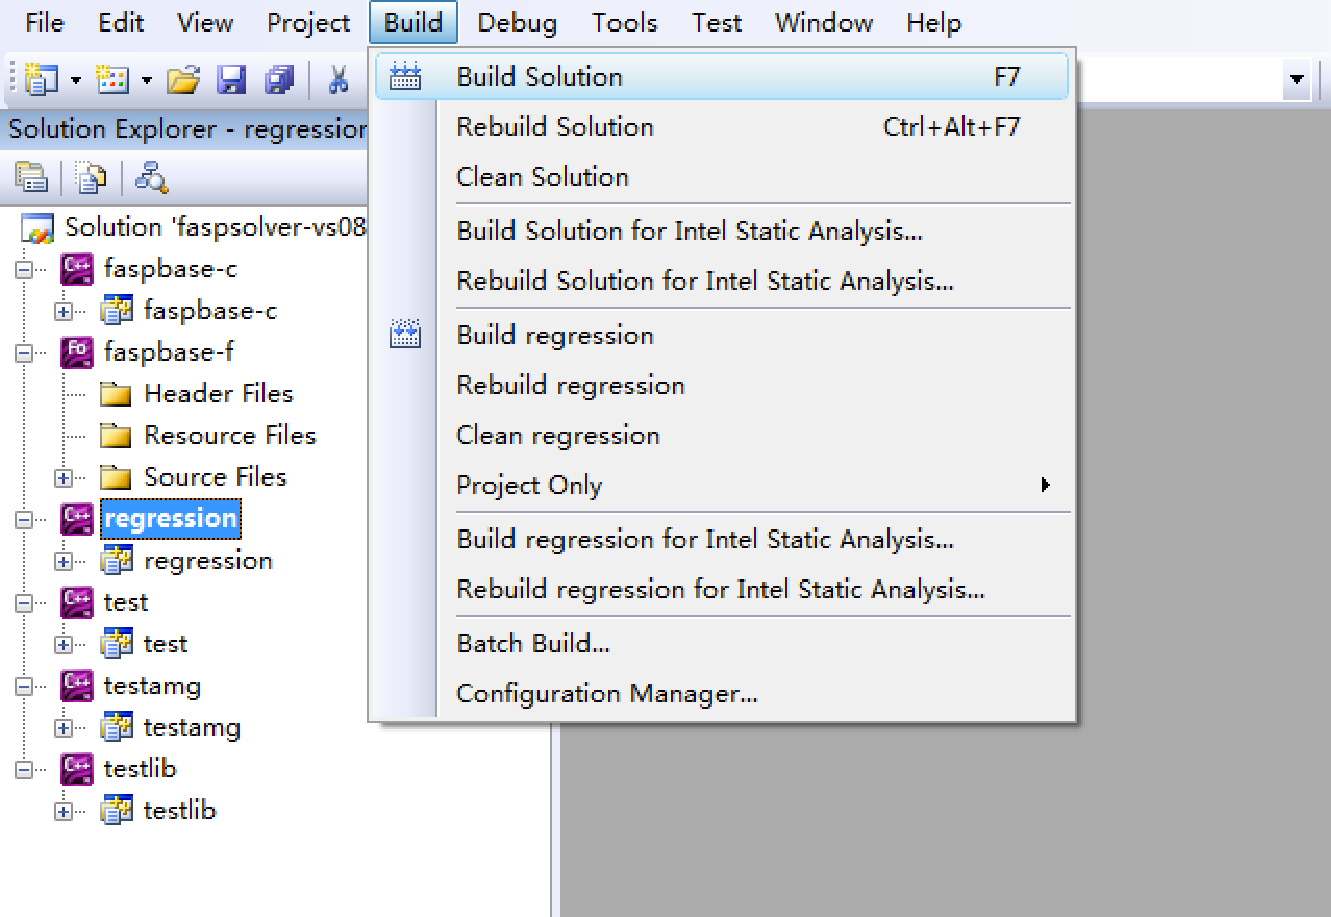
\includegraphics[width=0.9\linewidth]{fig/build-fasp.pdf} 
   \caption{Build FASP using Visual Studio 2008.}
   \label{fig:build}
\end{figure}


\begin{snugshade}\noindent
You need a C/C++ complier and a Fortran compiler together with Visual Studio to build FASP. You can use either Microsoft Visual C++ or Intel C compiler, together with Intel Fortran compiler.
\end{snugshade}

\begin{snugshade}\noindent
If you are using other versions of Visual Studio (like VS05 or VS12), do NOT convert the "VS08" solution file to your VS version because the FASP files might be cleaned up (removed) by Visual Studio automatically. You have to create another solution to build all the libraries and test programs by yourselves.
\end{snugshade}

If you need to build a VS solution by yourselves, you should create 5 projects:
\begin{enumerate}
\item ``faspbase-c'' contains all the ``.c'' and ``.inl'' files in the directory ``./base/src/''. You should add ``./base/include'' in Additional Directories. This project contains the core subroutines of faspsolver. 
\item ``faspbase-f'' contains all the ``.f'' files in ``./base/src/'' and ``./base/extra/sparsekit''. 
\item ``testlib'' contains all the ``.c'' files in ``./test/src/''. You should add ``./test/include'' in Additional Directories.
\item ``test'' is an executing program for test purpose in FASP. The source file is ``./test/main/test.c''.
\item ``regression'' is another executing program, which contains several methods to test the problems. The source file is ``./test/main/regression.c''.
\end{enumerate}

\begin{snugshade}\noindent
NOTE: If you are using Visual C++, all the C files should be compiled as C++ code (by using the /TP compiling option).
\end{snugshade}

After you successfully build the solution, you will get two static libraries named ``faspbase-c-vs08.lib'' and ``faspbase-f-vs08.lib''. You can use the ``lib'' command to wrap together as one single file (e.g. FASP.lib) for better portability. For example:
%
\begin{lstlisting}[numbers=none]
C:\FASP> lib /ltcg /out:FASP.lib faspbase-c-vs08.lib faspbase-f-vs08.lib
\end{lstlisting}
%

\subsection{Using GUI based on TCL}
You can also try to build FASP using the TCL graphical user interface. For example, in Linux or Mac OS X, you may 
%
\begin{lstlisting}[numbers=none]
$ wish FASP_install.tcl
\end{lstlisting}
%
A graphical interface will pop up and the rest of the building process is straightforward. 

\begin{comment}
\subsection{Using Scons}
In Linux, Mac OS X, or Windows, you can use the Scons tool to build and install different versions (Release, Shared, Debug) of the FASP library. You just need to type inside ``faspsolve/bas'' directory:
%
\begin{lstlisting}[numbers=none]
$ scons -Q install
\end{lstlisting}

By default, Scons will search for its preferred compilers in your system. If you wish to use your special compilers, you may use FC and CC flags to achieve this goal. For example, if a Windows user want to use Intel Fortran and VC++ compilers for FASP, he/she can use:
\begin{lstlisting}[numbers=none]
C:\> scons -Q install FC=ifort CC=cl
\end{lstlisting}

\begin{snugshade}\noindent
Usually, the directories for compilers are not added to the PATH environment variable automatically. Hence, you may need to modify your PATH variable to make the above line to work. 
\end{snugshade}
\end{comment}


\subsection{External libraries}\label{ssec:lib}

There are a few \emph{optional} external libraries that you might want to use, including memory allocation routines, direct solvers, ILU methods, discretization packages, etc. FASP has interfaces to a couple of them which we often use, for example, UMFPack, SuperLU, MUMPS, dlmalloc, SparseKit.


%%%%%%%%%%%%%%%%%%%%%%%%%%%%%%
\chapter{A Tutorial}\label{ch:tutor}
%%%%%%%%%%%%%%%%%%%%%%%%%%%%%%

In this chapter, we use a couple simple examples to demonstrate how to use the FASP package for solving existing linear systems which have been saved as disk files. All the examples can be found in ``faspsolver/tutorial/''. Here we only discuss the C version of these examples; interested users can read the F90 version of some of the examples. After you successfully build FASP (see \S\ref{sec:build}), just go to the ``faspsolver/tutorial/" directory and the compiled tutorial examples should be ready to be tried.

%%%%%%%%%%%%%%%%%%%%%%%%%%%%%%
\section{The first example}\label{sec:ex1}
%%%%%%%%%%%%%%%%%%%%%%%%%%%%%%

The first example is the simplest one that we can imagine: We read the stiffness matrix $A$ and right-hand side $b$ from disk files; then we solve $Ax=b$ using the classical AMG method~\cite{Brandt.BrandtMcCormick.1982uq,Ruge.RugeStuben.1985ij,Ruge.RugeStuben.1987bs}; see \S\ref{sec:amg}. The stiffness matrix $A$ is symmetric positive definite (SPD), arising from the continuous piecewise linear finite element discretization of the Poisson equation 
$$-\Delta u = f$$ 
(with the Dirichlet boundary condition) on a simple quasi-uniform triangulation of the bounded domain $\Omega$.
%
\lstinputlisting{../tutorial/main/poisson-amg.c}
%
Since this is the first example, we will explain it in some detail:
\begin{itemize}
%
\item Line 1 tells the Doxygen documentation system that the filename is ``poisson-amg.c''. Line 3--5 tells the Doxygen what is the purpose of this file (function). 
%
\item Line 12--13 includes the main FASP header file ``fasp.h'' and FASP function decoration header ``fasp\_functs.h''. These two headers shall be included in all files that requires FASP subroutines. Please also be noted that the function decorations in ``fasp\_functs.h'' is automatically generated from the source files and should NOT be modified by an enduser. 
%
\item Line 39 reads solver parameters from ``tutorial/ini/amg.dat''; see more discussions in \S\ref{sec:parameters}. In this disk file, we can set the location of the data files, type of solvers, maximal number of iteration numbers, convergence tolerance, and many other parameters for iterative solvers. Note that, in this function, we have initialize ``amgparam'' at the same time. 
%
\item Line 47 defines a sparse matrix $A$ in the compressed sparse row (CSR) format. Line 48 defines two vectors: the right-hand side $b$ and the numerical solution $x$. We refer to~\S\ref{sec:blas} for definitions of vectors and general sparse matrices.
%
\item Line 60 reads the matrix and the right-hand side from two disk files. Line 49--58 defines the filenames of them.
%
\item Line 63--67 prints basic information of coefficient matrix, right-hand side, and solver parameters.
%
\item Line 72--73 allocates memory for the solution vector $x$ and set its initial value to be all zero.
%
\item Line 75 solves $Ax=b$ using the AMG method. Type the AMG method and other parameters have been given in ``amgparam'' at Line 24; see \S\ref{sec:amg}.
%
\item Line 78--80 frees up memory allocated for $A$, $b$, and $x$.
\end{itemize}
%
To run this example, we can simply type (the default parameters have been in ``tutorial/ini/amg.dat'').
%
\begin{lstlisting}[numbers=none]
$ ./poisson-amg-c.ex
\end{lstlisting}
%
A sample output is given as follows (note that the actual output depends on the solver parameters and might be different than what you see here):
\begin{lstlisting}[numbers=none]
========================================
||   FASP: AMG example -- C version   ||
========================================

fasp_dcsrvec2_read: reading file ../data/csrmat_FE.dat...
fasp_dcsrvec2_read: reading file ../data/rhs_FE.dat...
A: m = 3969, n = 3969, nnz = 27281
b: n = 3969

       Parameters in AMG_param
-----------------------------------------------
AMG print level:                   3
AMG max num of iter:               100
AMG type:                          1
AMG tolerance:                     1.00e-08
AMG max levels:                    20
AMG cycle type:                    1
AMG scaling of coarse correction:  0
AMG smoother type:                 2
AMG smoother order:                1
AMG num of presmoothing:           2
AMG num of postsmoothing:          2
AMG coarsening type:               1
AMG interpolation type:            1
AMG dof on coarsest grid:          500
AMG strong threshold:              0.6000
AMG truncation threshold:          0.4000
AMG max row sum:                   0.9000
AMG aggressive levels:             0
AMG aggressive path:               1
-----------------------------------------------


Calling classical AMG ...
-----------------------------------------------
  Level     Num of rows      Num of nonzeros
-----------------------------------------------
    0            3969             27281
    1            1985             28523
    2             961             20519
    3             481             13153
-----------------------------------------------
AMG grid complexity     = 1.863
AMG operator complexity = 3.280
Classical AMG setup costs 0.0123 seconds.
-----------------------------------------------------------
It Num |   ||r||/||b||   |     ||r||      |  Conv. Factor
-----------------------------------------------------------
     0 |  1.000000e+00   |  7.514358e+00  |     -.--
     1 |  5.160015e-04   |  3.877420e-03  |     0.0005
     2 |  1.895524e-06   |  1.424365e-05  |     0.0037
     3 |  7.554832e-09   |  5.676972e-08  |     0.0040
Number of iterations = 3 with relative residual 7.554832e-09.
AMG solve costs 0.0189 seconds.
AMG totally costs 0.0316 seconds.
\end{lstlisting}



%%%%%%%%%%%%%%%%%%%%%%%%%%%%%%
\section{The second example}\label{sec:ex2}
%%%%%%%%%%%%%%%%%%%%%%%%%%%%%%

In the second example, we modify the previous example slightly and solve the Poisson equation using iterative methods.
%
\lstinputlisting{../tutorial/main/poisson-its.c}
%
This example is very similar to the first example and we briefly explain the differences:
\begin{itemize}
%
\item Line 37 is slightly different than Line 39 in the previous example---Instead of initializing ``amgparam'', we initialize ``itparam''. This is because we are calling general interface of Krylov subspace methods~\cite{Saad.Saad.2003fv} and the parameters are recorded in ``itparam''.
%
\item Line 70--71 allocates memory for the solution vector $x$ and set its initial value to be all zero.
%
\item Line 73 solves $Ax=b$ using the general interface for Krylov subspace methods. Type the iterative method and other parameters have been specified in ``itparam''; see \S\ref{sec:iter} for details.
%
\end{itemize}
%
To run this example, we can simply type (the default parameters have been in ``tutorial/ini/its.dat'').
%
\begin{lstlisting}[numbers=none]
$ ./poisson-its-c.ex
\end{lstlisting}

%%%%%%%%%%%%%%%%%%%%%%%%%%%%%%
\section{The third example}\label{sec:ex3}
%%%%%%%%%%%%%%%%%%%%%%%%%%%%%%

This example is slightly longer and is a modification of the previous one. In this example,  we wish to demonstrate how to setup a simple preconditioner for the preconditioned conjugate gradient (PCG) method.
%
\lstinputlisting{../tutorial/main/poisson-pcg.c}
%
This example is very similar to the first example and we now briefly explain it:
\begin{itemize}
%
\item Line 40 reads parameters from ``tutorial/ini/pcg.dat''. In this example, we need parameters for iterative methods, AMG preconditioner, and ILU preconditioner. The type of the preconditioner is also set in ``pcg.dat'' and recorded in ``pc\_type''; see Line 30 in ``pcg.dat''.
%
\item Line 76 sets up the desired preconditioner and prepare it for the preconditioned iterative methods.
%
\item Line 86 calls PCG to solve $Ax=b$. One can also call the general iterative method interface as in the previous example.
%
\item Line 89 cleans up auxiliary data associated with the preconditioner in use if necessary. 
%
\end{itemize}
%
To run this example, we can simply type (the default parameters have been in ``tutorial/ini/pcg.dat'').
%
\begin{lstlisting}[numbers=none]
$ ./poisson-pcg-c.ex
\end{lstlisting}


%%%%%%%%%%%%%%%%%%%%%%%%%%%%%%
\section{Set parameters}\label{sec:parameters}
%%%%%%%%%%%%%%%%%%%%%%%%%%%%%%

In the previous examples, we have seen how to read input parameters from disk files. Now we take a brief look inside those ini files. We take ``tutorial/ini/amg.dat'' as an example:
%
\begin{lstlisting}
%----------------------------------------------%
% input parameters                             %
% lines starting with % are comments           %
% must have spaces around the equal sign "="   %
%----------------------------------------------%

workdir = ../data/    % work directory, no more than 128 characters
print_level = 3       % How much information to print out

%----------------------------------------------%
% parameters for multilevel iteration          %
%----------------------------------------------%

AMG_type                 = C      % C classic AMG
                                  % SA smoothed aggregation
                                  % UA unsmoothed aggregation
AMG_cycle_type           = V      % V V-cycle | W W-cycle
                                  % A AMLI-cycle | NA Nonlinear AMLI-cycleA
AMG_tol                  = 1e-8   % tolerance for AMG
AMG_maxit                = 100    % number of AMG iterations
AMG_levels               = 20     % max number of levels
AMG_coarse_dof           = 500    % max number of coarse degrees of freedom
AMG_coarse_scaling       = OFF    % switch of scaling of the coarse grid correction
AMG_amli_degree          = 2      % degree of the polynomial used by AMLI cycle
AMG_nl_amli_krylov_type  = 6      % Krylov method in NLAMLI cycle: 6 FGMRES | 7 GCG

%----------------------------------------------%
% parameters for AMG smoothing                 %
%----------------------------------------------%

AMG_smoother             = GS     % GS | JACOBI | SGS
                                  % SOR | SSOR | GSOR | SGSOR | POLY
AMG_ILU_levels           = 0      % number of levels using ILU smoother
AMG_schwarz_levels       = 0      % number of levels using Schwarz smoother
AMG_relaxation           = 1.1    % relaxation parameter for SOR smoother
AMG_polynomial_degree    = 3      % degree of the polynomial smoother
AMG_presmooth_iter       = 2      % number of presmoothing sweeps
AMG_postsmooth_iter      = 2      % number of postsmoothing sweeps

%----------------------------------------------%
% parameters for classical AMG SETUP           %
%----------------------------------------------%

AMG_coarsening_type      = 1      % 1 Modified RS
                                  % 3 Compatible Relaxation
                                  % 4 Aggressive
AMG_interpolation_type   = 1      % 1 Direct | 2 Standard | 3 Energy-min
AMG_strong_threshold     = 0.6    % Strong threshold
AMG_truncation_threshold = 0.4    % Truncation threshold
AMG_max_row_sum          = 0.9    % Max row sum

%----------------------------------------------%
% parameters for aggregation-type AMG SETUP    %
%----------------------------------------------%

AMG_strong_coupled       = 0.08   % Strong coupled threshold
AMG_max_aggregation      = 20     % Max size of aggregations
AMG_tentative_smooth     = 0.67   % Smoothing factor for tentative prolongation
AMG_smooth_filter        = OFF    % Switch for filtered matrix for smoothing\end{lstlisting}
%
We now briefly discuss the parameters above:
%
This example is very similar to the first example and we now briefly explain it:
\begin{itemize}
%
\item Line 7 sets the working directory, which should contain data files for the matrices (and right-hand side vectors when necessary).
%
\item Line 8 sets the level of output for FASP routines. It should range from 0 to 10 with 0 means no output and 10 means output everything possible.
%
\item Line 14--25 sets the basic parameters for multilevel iterations. For example, type of AMG, type of multilevel cycles, number of maximal levels, etc.
%
\item Line 31--38 sets the type of smoothers, number of smoothing sweeps, etc.
%
\item Line 44--50 sets the parameters for the setup phase of the classical AMG method (\S\ref{sec:amg}).
%
\item Line 56--59 gives the parameters for the setup phase of the aggregation-base AMG methods (\S\ref{sec:amg}).
%
\end{itemize}
%

You can do a very simple experiment and change the AMG type from the classical AMG to smoothed aggregation AMG by revise Line 14 to
%
\begin{lstlisting}[numbers=none]
AMG_type                 = SA
\end{lstlisting}
%
Then you run ``poisson-amg-c.ex'' one more time and will get
%
\begin{lstlisting}[numbers=none]
========================================
||   FASP: AMG example -- C version   ||
========================================

fasp_dcsrvec2_read: reading file ../data/csrmat_FE.dat...
fasp_dcsrvec2_read: reading file ../data/rhs_FE.dat...
A: m = 3969, n = 3969, nnz = 27281
b: n = 3969

       Parameters in AMG_param
-----------------------------------------------
AMG print level:                   3
AMG max num of iter:               100
AMG type:                          2
AMG tolerance:                     1.00e-08
AMG max levels:                    20
AMG cycle type:                    1
AMG scaling of coarse correction:  0
AMG smoother type:                 2
AMG smoother order:                1
AMG num of presmoothing:           2
AMG num of postsmoothing:          2
Aggregation AMG strong coupling:   0.0800
Aggregation AMG max aggregation:   20
Aggregation AMG tentative smooth:  0.6700
Aggregation AMG smooth filter:     0
-----------------------------------------------


Calling SA AMG ...
-----------------------------------------------
  Level     Num of rows      Num of nonzeros
-----------------------------------------------
    0            3969             27281
    1             541              6531
    2              41               421
-----------------------------------------------
AMG grid complexity     = 1.147
AMG operator complexity = 1.255
Smoothed aggregation setup costs 0.0072 seconds.
-----------------------------------------------------------
It Num |   ||r||/||b||   |     ||r||      |  Conv. Factor
-----------------------------------------------------------
     0 |  1.000000e+00   |  7.514358e+00  |     -.--
     1 |  4.345463e-02   |  3.265336e-01  |     0.0435
     2 |  8.041967e-03   |  6.043022e-02  |     0.1851
     3 |  3.808810e-03   |  2.862076e-02  |     0.4736
     4 |  1.838990e-03   |  1.381883e-02  |     0.4828
     5 |  8.675952e-04   |  6.519421e-03  |     0.4718
     6 |  4.089274e-04   |  3.072827e-03  |     0.4713
     7 |  1.939823e-04   |  1.457653e-03  |     0.4744
     8 |  9.276723e-05   |  6.970862e-04  |     0.4782
     9 |  4.471799e-05   |  3.360270e-04  |     0.4820
    10 |  2.171249e-05   |  1.631554e-04  |     0.4855
    11 |  1.060934e-05   |  7.972239e-05  |     0.4886
    12 |  5.212246e-06   |  3.916668e-05  |     0.4913
    13 |  2.572464e-06   |  1.933042e-05  |     0.4935
    14 |  1.274466e-06   |  9.576797e-06  |     0.4954
    15 |  6.333891e-07   |  4.759512e-06  |     0.4970
    16 |  3.155926e-07   |  2.371476e-06  |     0.4983
    17 |  1.575755e-07   |  1.184079e-06  |     0.4993
    18 |  7.881043e-08   |  5.922098e-07  |     0.5001
    19 |  3.947044e-08   |  2.965950e-07  |     0.5008
    20 |  1.978978e-08   |  1.487075e-07  |     0.5014
    21 |  9.931176e-09   |  7.462641e-08  |     0.5018
Number of iterations = 21 with relative residual 9.931176e-09.
AMG solve costs 0.0252 seconds.
AMG totally costs 0.0327 seconds.
\end{lstlisting}
%
You can compare this with the sample results in \S\ref{sec:ex1}.

\begin{snugshade}\noindent
The input parameters allowed in FASP are not limited to the ones listed in this example. A list of possible iterative methods and preconditioners can be found in ``base/include/messages.h''; see \S\ref{sec:const}. For more parameters and their ranges, we refer to the Reference Manual.
\end{snugshade}

%%%%%%%%%%%%%%%%%%%%%%%%%%%%%%
\chapter{Basic Usage}\label{ch:basic}
%%%%%%%%%%%%%%%%%%%%%%%%%%%%%%

In this chapter, we discuss the basic data structures and important building blocks which will be useful later for constructing auxiliary space preconditioners for systems of PDEs in Chapter~\ref{ch:advanced}. In particular, we will discuss vectors, sparse matrices, iterative methods, and multigrid methods.

%%%%%%%%%%%%%%%%%%%%%%%%%%%%%%
\section{Vectors and sparse matrices}\label{sec:blas}
%%%%%%%%%%%%%%%%%%%%%%%%%%%%%%

The most important data structures for iterative methods are probably vectors and sparse matrices. In this section, we first discuss the data structures for vectors and matrices in FASP; and then we discuss BLAS for sparse matrices.

\subsection{Vectors}

The data structure for vectors is very simple. It only contains the length of the vector and an array which contains the entries of this vector.

\begin{lstlisting}
/**
 * \struct dvector
 * \brief Vector with n entries of REAL type.
 */
typedef struct dvector{
	
    //! number of rows
	INT row;
    //! actual vector entries
	REAL *val;
	
} dvector; /**< Vector of REAL type */
\end{lstlisting}

\subsection{Sparse matrices}

On the other hand, sparse matrices for PDE applications are very complicated. It depends on the particular applications, discretization methods, as well as solution algorithms. In FASP, there are several types of sparse matrices, COO, CSR, CSRL, BSR, and CSR Block, etc. The presentation closely follows ideas from Pissanetzky~\cite{Pissanetzky.Pissanetzky.1984hc}.

In this section, we use the following sparse matrix as an example to explain different formats for sparse matrices:
%
\begin{example}\label{ex:sparse}
Consider the following $4\times 5$ matrix with 12 non-zero entries
$$
\left(\begin{array}{ccccc}
1 & 1.5 & 0 & 0 & 12\\
0 & 1    & 6 & 7 & 1\\
3 & 0    & 6 & 0 & 0\\
1 & 0    & 2 & 0 & 5
\end{array}
\right)
$$
\end{example}

\subsubsection*{(i) COO format}

The coordinate (COO) format or IJ format is the simplest sparse matrix format.
\begin{lstlisting}
/**
 * \struct dCOOmat
 * \brief Sparse matrix of REAL type in COO (or IJ) format.
 *
 * Coordinate Format (I,J,A)
 *
 * \note The starting index of A is 0.
 */
typedef struct dCOOmat{
	
	//! row number of matrix A, m
	INT row;
	//! column of matrix A, n
	INT col;
	//! number of nonzero entries
	INT nnz;
	//! integer array of row indices, the size is nnz
	INT *I;
	//! integer array of column indices, the size is nnz
	INT *J;
	//! nonzero entries of A
	REAL *val;
	
} dCOOmat; /**< Sparse matrix of REAL type in COO format */
\end{lstlisting}
%
So it clear that the sparse matrix in Example~\ref{ex:sparse} in COO format is stored as:
%
\begin{lstlisting}[numbers=none]
row = 4
col = 5
nnz = 12

 I J  val
-----------
 0 0  1.0
 0 1  1.5
 0 4 12.0
 1 1  1.0
 1 2  6.0
 1 3  7.0
 1 4  1.0
 .......
\end{lstlisting}
%
Although the COO format is easy to understand or use, it wastes storage space and has little advantages in sparse BLAS operations.

\begin{snugshade}\noindent
NOTE: In FASP, the indices always start from 0, instead of from 1. This is often the source of problems related to vectors and matrices.
\end{snugshade}

\subsubsection*{(ii) CSR format}
The most commonly used data structure for sparse matrices nowadays is probably the so-called {\em compressed sparse row}  (CSR) format, according to Saad~\cite{Saad.Saad.2003fv}. The compressed row storage format of a matrix $A\in \mathbb{R}^{n\times m}$ ($n$ rows and $m$ columns) consists of three arrays, as follows:
%
\begin{enumerate}
\item An integer array of row pointers of size n+1;
\item An integer array of column indexes of size nnz;
\item An array of actual matrix entries.
\end{enumerate}
%
In FASP, we define:
\begin{lstlisting}
/**
 * \struct dCSRmat
 * \brief Sparse matrix of REAL type in CSR format.
 *
 * CSR Format (IA,JA,A) in REAL
 *
 * \note The starting index of A is 0.
 */
typedef struct dCSRmat{
	
	//! row number of matrix A, m
	INT row;
	//! column of matrix A, n
	INT col;
	//! number of nonzero entries
	INT nnz;
	//! integer array of row pointers, the size is m+1
	INT *IA;
	//! integer array of column indexes, the size is nnz
	INT *JA;
	//! nonzero entries of A
	REAL *val;
	
} dCSRmat; /**< Sparse matrix of REAL type in CSR format */
\end{lstlisting}
%
The matrix ({only nonzero elements}) is stored in the array $val$
row after row, in a way that $i$-th row begins at $val(IA(i))$ and ends
at $val(IA(i+1)-1)$. In the same way, $JA(IA(i)$ to $JA(IA(i+1)-1)$ will
contain the column indexes of the non-zeros in row $i$. Thus $IA$ is of
size $n+1$ (number of rows in $val$ plus one), $JA$ and $val$ are of size
equal to the number of non-zeroes. The total number of non-zeroes is
equal to $IA(n+1)-1$.

\begin{snugshade}\noindent
NOTE: When the sparse matrix $A$ is a boolean (i.e. all entries are either $0$ or
$1$), the actual non-zeroes are not stored because it is understood that, if it is
nonzero, it could only be $1$ and there is no need to store it.
\end{snugshade}

The matrix in Example~\ref{ex:sparse} in CSR format is represented in the following way:
\begin{itemize}
\item $IA$ is of size $5$ and
$$IA =
\begin{array}{||c||c||c||c||c||}0&3&7&9&12\end{array}
$$
\item $JA$ is of size $IA(5)-1=12$
$$JA =
\begin{array}{||c|c|c||c|c|c|c||c|c||c|c|c||}
0&1&4&1&3&2&4&0&2&2&4&0
\end{array}
$$
\item $val$ is of the same size as $JA$ and
$$val =
\begin{array}{||c|c|c||c|c|c|c||c|c||c|c|c||}
1.&1.5&12.&1.&7.&6.&1.&3.&6.&2.&5.&1.
\end{array}
$$
\end{itemize}
Here we use double vertical bars to separate rows and single vertical bars to separate values.

\begin{snugshade}\noindent
NOTE: The indices in $JA$ and entries of $val$ does NOT have to be ordered as seen in this example. Sometimes they are sorted in ascending order in each row. More often, the diagonal entries are stored in the first position in each row and the rest are sorted in ascending order.
\end{snugshade}

Below is a ``non-numeric'' example.
%
\begin{example} Consider the following sparse matrix:
$$
\left(
\begin{array}{cccc}
a_{11} & 0 & a_{13} & 0 \\
0 & a_{22} & a_{23} & a_{24} \\
0 & a_{32} & 0 & a_{34} \\
a_{41}& a_{42} & a_{43} & 0 \\
\end{array}
\right)
$$
For this matrix, we have that the number of non-zeros $nnz=10$. Furthermore, the three arrays of in the CSR format are:
$$
IA =
\begin{array}{||c||c||c||c||}0&2&5&7\end{array}\, ,
%[ 0 \quad 2 \quad 5 \quad 7 \quad 10],
$$
$$
JA =
\begin{array}{||c|c||c|c|c||c|c||c|c|c||}
0&2&1&2&3&1&3&0&1&2\end{array}\, ,
%[ 0 \; 2 \;|\; 1 \; 2 \; 3 \;|\; 1 \; 3 \;|\; 0 \; 1 \; 2],
$$
and
$$
val =
\begin{array}{||c|c||c|c|c||c|c||c|c|c||}
a_{11} & a_{13} & a_{22} & a_{23} & a_{24} & a_{32} & a_{34} & a_{41} & a_{42} & a_{43}\end{array}\,.
%[a_{11} \; a_{13}\;|\; a_{22} \; a_{23} \; a_{24}\;|\; a_{32} \; a_{34}\;|\; a_{41}\; a_{42}\; a_{43}].
$$
\end{example}

\begin{snugshade}\noindent
NOTE: The CSR format presents challenges to sparse matrix-vector product mainly because of the high cache missing rate due to indirect memory access and irregular access pattern. In order to reduce the cache missing rate, we introduce an improved data format, CSRL.
\end{snugshade}

\subsubsection*{(iii) CSRL format}

CSRL matrix format~\cite{Mellor-crummey2004} groups rows with same number of nonzeros together and improves cache hitting rate.
\begin{lstlisting}
/*!
 * \struct dCSRLmat
 * \brief Sparse matrix of REAL type in CSRL format.
 */
typedef struct dCSRLmat{

	//! number of rows	
	INT row;
	//! number of cols
	INT col;
	//! number of nonzero entries
	INT nnz;
	//! number of different values in i-th row, i=0:nrows-1
	INT dif;
	//! nz_diff[i]: the i-th different value in 'nzrow'
	INT *nz_diff;
	//! row index of the matrix (length-grouped): rows with same nnz are together
	INT *index;
	//! j in {start[i],...,start[i+1]-1} means nz_diff[i] nnz in index[j]-row	
	INT *start;
	//! column indices of all the nonzeros
	INT *ja;
	//! values of all the nonzero entries
	REAL *val;

} dCSRLmat; /**< Sparse matrix of REAL type in CSRL format */
\end{lstlisting}

\section{Block sparse matrices}

For PDE applications, we often need to solve systems of partial differential equations. Many iterative methods and preconditioners could take advantages of the structure of PDE systems and improve efficiency. So we often need to use semi-structured (block) sparse data structures to store the coefficient matrix arising from PDE systems. 

Depending on different applications and different solving algorithms, we can use two types of block matrices: dBSRmat (or BSR Block Compressed Sparse Row) and block\_dCSRmat (CSR Block or Block of CSR matrices). 

\begin{snugshade}\noindent
For more details as well as other specialized block matrices, readers are referred to the header file ``base/include/fasp\_block.h''.
\end{snugshade}

As an example, we consider the following matrix, which have been used in \S\ref{sec:blas} for the CSR format. We add structure to this matrix and divide it as a $2 \times 2$ block matrix:
%
\begin{example}\label{ex:block}
$$
\left(
\begin{array}{cc|cc}
a_{11} & 0 & a_{13} & 0 \\
0 & a_{22} & a_{23} & a_{24} \\
\hline
0 & a_{32} & 0 & a_{34} \\
a_{41}& a_{42} & a_{43} & 0 \\
\end{array}
\right)
$$
\end{example}

\subsubsection*{(i) BSR format}
This format is a standard data structure for storing block sparse matrices which has been used by the Intel MKL library. 

\begin{lstlisting}
/**
 * \struct dBSRmat
 * \brief Block sparse row storage matrix of REAL type.
 *
 * \note This data structure is adapted from the Intel MKL library.
 * Refer to
 * http://software.intel.com/sites/products/documentation/hpc/mkl/lin/index.htm
 *
 * \note Some of the following entries are capitalized to stress that they are
 *       for blocks!
 *
 */
typedef struct dBSRmat{
	

	//! number of rows of sub-blocks in matrix A, M
	INT ROW;
	//! number of cols of sub-blocks in matrix A, N
	INT COL;
	//! number of nonzero sub-blocks in matrix A, NNZ
	INT NNZ;
	//! dimension of each sub-block
	INT nb; // for the moment, allow nb*nb full block
	//! storage manner for each sub-block
	INT storage_manner; // 0: row-major order, 1: column-major order
	
	//! A real array that contains the elements of the non-zero blocks of
	//! a sparse matrix. The elements are stored block-by-block in row major
	//! order. A non-zero block is the block that contains at least one non-zero
	//! element. All elements of non-zero blocks are stored, even if some of
	//! them is equal to zero. Within each nonzero block elements are stored
	//! in row-major order and the size is (NNZ*nb*nb).
	REAL *val;
	
	//! integer array of row pointers, the size is ROW+1
	INT *IA;
	
	//! Element i of the integer array columns is the number of the column in the
	//! block matrix that contains the i-th non-zero block. The size is NNZ.
	INT *JA;
	
} dBSRmat; /**< Matrix of REAL type in BSR format */
\end{lstlisting}

For the matrix in Example~\ref{ex:block}, we have that the number of block rows $ROW=2$, the number of block columns $COL=2$, and the number of block nonzeros $NNZ = 4$. The block size is $nb = 2$. We can choose different storage manners for storing the small blocks. Suppose that we set it to be 0, i.e. row-major format. Then the three arrays of in the BSR format are:
$$
IA =
\begin{array}{||c||c||c||c||}0&8&16\end{array}\, ,
$$
$$
JA =
\begin{array}{||c|c||c|c||}
0&1&0&1\end{array}\, ,
$$
and
\begin{align*}
val = \;\; &
\begin{array}{||c|c|c|c||c|c|c|c||}
a_{11} & 0 & 0 & a_{22} & a_{13} & 0 & a_{23} & a_{24}
\end{array}\,
\\
& \begin{array}{||c|c|c|c||c|c|c|c||}
0 & a_{32} & a_{41} & a_{42} & 0 & a_{34} & a_{43} & 0
\end{array}\,.
\end{align*}
We immediately notice that this format might be not be the best choice for this particular matrix due to all the blocks are nonzero blocks, i.e., contain nonzero entries. However, for PDE applications, this does not usually happen. 

\subsubsection*{(ii) CSR Block format}
This format is simple and is derived from the dCSRmat data structure. The following definition explains itself. 
\begin{lstlisting}
/**
 * \struct block_dCSRmat
 * \brief Block of REAL CSR matrix structure.
 *
 * CSR Block Format in REAL
 *
 * \note The starting index of A is 0.
 */
typedef struct block_dCSRmat{
	
	//! row number of blocks in A, m
	INT brow;
	//! column number of blocks A, n
	INT bcol;
	//! blocks of dCSRmat, point to blocks[brow][bcol]
	dCSRmat **blocks;
	
} block_dCSRmat; /**< Matrix of REAL type in Block BSR format */
\end{lstlisting}
%


\section{I/O subroutines for sparse matrices}

To be added.


\section{Sparse BLAS}

The matrix-vector multiplication: $y=Ax$ can be performed in the
following simple way:

\begin{lstlisting}
/**
 * \fn void fasp_blas_dcsr_mxv (dCSRmat *A, REAL *x, REAL *y)
 *
 * \brief Matrix-vector multiplication y = A*x
 *
 * \param A   Pointer to dCSRmat matrix A
 * \param x   Pointer to array x
 * \param y   Pointer to array y
 *
 * \author Chensong Zhang
 * \date   07/01/2009
 */
void fasp_blas_dcsr_mxv (dCSRmat *A,
                         REAL *x,
                         REAL *y)
{
    const INT   m  = A->row;
    const INT  *ia = A->IA, *ja = A->JA;
    const REAL *aj = A->val;

    INT i, k, beg, end;
    register REAL tmp;

    for ( i=0; i<m; ++i ) {
        tmp = 0.0;
        beg = ia[i]; end = ia[i+1];
        for ( k=beg; k<end; ++k ) tmp += aj[k]*x[ja[k]];
        y[i] = tmp;
    }
}
\end{lstlisting}

This is only a simple example for sparse matrix-vector multiplication (SpMV) kernel. Since we need many types of sparse matrices, there are various of versions of SpMV for different data structures. See the Reference Manual for more details.

%%%%%%%%%%%%%%%%%%%%%%%%%%%%%%
\section{Iterative methods}\label{sec:iter}
%%%%%%%%%%%%%%%%%%%%%%%%%%%%%%

In FASP, there are a couple of standard preconditioned iterative methods
~\cite{Saad.Saad.2003fv} implemented, including preconditioned CG, BiCGstab, GMRES, Variable Restarting GMRES, Flexible GMRES, etc. In this section, we use the CSR matrix format as example to introduce how to call these iterative methods. To learn more details, we refer to the Reference Manual.

We first notice the abstract interface for the iterative methods is:
%
\begin{lstlisting}[numbers=none]
/**
 * \fn INT fasp_solver_dcsr_itsolver (dCSRmat *A, dvector *b, dvector *x,
 *                                    precond *pc, itsolver_param *itparam)
 *
 * \brief Solve Ax=b by preconditioned Krylov methods for CSR matrices
 *
 * \param A        Pointer to the coeff matrix in dCSRmat format
 * \param b        Pointer to the right hand side in dvector format
 * \param x        Pointer to the approx solution in dvector format
 * \param pc       Pointer to the preconditioning action
 * \param itparam  Pointer to parameters for iterative solvers
 *
 * \return         Number of iterations if succeed
 *
 * \author Chensong Zhang
 * \date   09/25/2009
 *
 * \note This is an abstract interface for iterative methods.
 */
INT fasp_solver_dcsr_itsolver (dCSRmat *A,
                               dvector *b,
                               dvector *x,
                               precond *pc,
                               itsolver_param *itparam)
\end{lstlisting}
%
The names of the input arguments explain themselves mostly and they are explained in the Reference Manual in detail.

We briefly discuss how to call this function; and, once you understand PCG, you can easily call other iterative methods. The following code segment is taken from ``base/src/itsolver\_csr.c'':
%
\begin{lstlisting}
... ...

    // ILU setup for whole matrix
    ILU_data LU;
    if ( (status = fasp_ilu_dcsr_setup(A,&LU,iluparam))<0 ) goto FINISHED;

    // check iludata
    if ( (status = fasp_mem_iludata_check(&LU))<0 ) goto FINISHED;

    // set preconditioner
    precond pc;
    pc.data = &LU;
    pc.fct  = fasp_precond_ilu;

    // call iterative solver
    status = fasp_solver_dcsr_itsolver(A,b,x,&pc,itparam);

... ...
\end{lstlisting}
%
Now we explain this code segment a little bit:
\begin{itemize}
\item Line 3--4 performs the setup phase for ILU method. The particular type of ILU method is determined by ``iluparam''; see \S\ref{sec:parameters}. Line 7 performs a simple memory check for ILU.
\item Line 10--12 defines the preconditioner data structure ``pc'', which contains two parts: one is the actual preconditioning action ``pc.fct'', the other is the auxiliary data which is needed to perform the preconditioning action ``pc.data''.
\item Line 15 calls iterative methods. ``A'' is the matrix in dCSRmat format; ``b'' and ``x'' are the right-hand side and the solution vectors, respectively. Similar to ILU setup, the type of iterative methods is determined by ``itparam''.
\end{itemize}

Apparently, we now left with no choice but introducing ``itparam''.
\begin{lstlisting}[numbers=none]
/**
 * \struct itsolver_param
 * \brief Parameters passed to iterative solvers.
 *
 */
typedef struct {
	
	SHORT itsolver_type; /**< solver type: see message.h */
	SHORT precond_type;  /**< preconditioner type: see message.h */
	SHORT stop_type;     /**< stopping criteria type */
	INT   maxit;         /**< max number of iterations */
	REAL  tol;           /**< convergence tolerance */
	INT   restart;       /**< number of steps for restarting: for GMRES etc */
	SHORT print_level;   /**< print level: 0--10 */	
	
} itsolver_param; /**< Parameters for iterative solvers */
\end{lstlisting}
%
Possible ``itsolver\_type'' includes:
\begin{lstlisting}[numbers=none]
/**
 * \brief Definition of solver types for iterative methods
 */
#define SOLVER_CG               1    /**< Conjugate Gradient */
#define SOLVER_BiCGstab         2    /**< Biconjugate Gradient Stabilized */
#define SOLVER_MinRes           3    /**< Minimal Residual */
#define SOLVER_GMRES            4    /**< Generalized Minimal Residual */
#define SOLVER_VGMRES           5    /**< Variable Restarting GMRES */
#define SOLVER_VFGMRES          6    /**< Variable Restarting Flexible GMRES */
#define SOLVER_GCG              7    /**< Generalized Conjugate Gradient */
#define SOLVER_AMG              21   /**< AMG as an iterative solver */
#define SOLVER_FMG		        22   /**< Full AMG as an solver */
\end{lstlisting}


%%%%%%%%%%%%%%%%%%%%%%%%%%%%%%
\section{Geometric multigrid}\label{sec:gmg}
%%%%%%%%%%%%%%%%%%%%%%%%%%%%%%

To be added.

%%%%%%%%%%%%%%%%%%%%%%%%%%%%%%
\section{Algebraic multigrid}\label{sec:amg}
%%%%%%%%%%%%%%%%%%%%%%%%%%%%%%

The classical algebraic multigrid method~\cite{Ruge.RugeStuben.1987bs} is an important component in many of our auxiliary space preconditioners. Because of its user-friendly and scalability, AMG becomes increasingly popular in scientific and engineering computing, especially when GMG is difficult or not possible to be applied. Various of new AMG techniques~\cite{Vanek.VanekMandel.1996kl,Wan.WanChan.2000qa,Brezina.BrezinaCleary.2000ly,Henson.HensonVassilevski.2001cr,Chartier.ChartierFalgout.2003ve,Livne.Livne.2004kl,Falgout.FalgoutVassilevski.2004bh,Xu.XuZikatanov.2004pi,Brannick.BrannickZikatanov.2007zr,Muresan.MuresanNotay.2008tg, Hu.X;Vassilevski.P;Xu.J.2013a} have emerged in recent years.

The following code segment is part of ``base/src/amg.c'' and it is a good example which shows how to call different AMG methods (classical AMG, smoothed aggregation, un-smoothed aggregation) and different multilevel iterative methods (V-cycle, W-cycle, AMLI-cycle, Nonlinear AMLI-cycle, etc).
%
\begin{lstlisting}
... ...

    // param is a pointer to AMG_param
    const SHORT   max_levels  = param->max_levels;
    const SHORT   amg_type    = param->AMG_type;
    const SHORT   cycle_type  = param->cycle_type;

    // initialize mgl[0] with A, b, x
    AMG_data *mgl = fasp_amg_data_create(max_levels);
    mgl[0].A = fasp_dcsr_create(m,n,nnz); fasp_dcsr_cp(A,&mgl[0].A);
    mgl[0].b = fasp_dvec_create(n);       fasp_dvec_cp(b,&mgl[0].b);
    mgl[0].x = fasp_dvec_create(n);       fasp_dvec_cp(x,&mgl[0].x);

    // AMG setup phase
    switch (amg_type) {

    case SA_AMG: // Smoothed Aggregation AMG setup phase
        if ( (status=fasp_amg_setup_sa(mgl, param)) < 0 ) goto FINISHED;
        break;

    case UA_AMG: // Unsmoothed Aggregation AMG setup phase
        if ( (status=fasp_amg_setup_ua(mgl, param)) < 0 ) goto FINISHED;
        break;

    default: // Classical AMG setup phase
        if ( (status=fasp_amg_setup_rs(mgl, param)) < 0 ) goto FINISHED;
        break;

    }

    // AMG solve phase
    switch (cycle_type) {

    case AMLI_CYCLE: // call AMLI-cycle
        if ( (status=fasp_amg_solve_amli(mgl, param)) < 0 ) goto FINISHED;
        break;

    case NL_AMLI_CYCLE: // call Nonlinear AMLI-cycle
        if ( (status=fasp_amg_solve_nl_amli(mgl, param)) < 0 ) goto FINISHED;
        break;

    default: // call classical V,W-cycles
        if ( (status=fasp_amg_solve(mgl, param)) < 0 ) goto FINISHED;
        break;

    }

... ...
\end{lstlisting}
%
The code above is very simple and we only wish to point out that:
%
\begin{itemize}
\item Line 4--6 reads some of the parameters from ``AMG\_param'', which can be defined from a input file; see \S\ref{sec:parameters}.
\item Line 9--12 initializes the ``AMG\_data'' with a copy of the coefficient matrix, the right-hand side, and the initial solution (it will store the final solution eventually).
\item Line 17--27 calls three different AMG methods, determined by ``amg\_type''.
\item Line 34--44 calls three different multilevel iterative methods, determined by ``cycle\_type''.
\end{itemize}

\subsection{Parameters for AMG}

There are a couple of controlling parameters for algebraic multigrid methods in FASP. Basically, there are four types of parameters for AMG---They control multilevel iterations, smoothing, classical AMG setup, and aggregation AMG setup. The following is a sample from ``test/ini/input.dat'' and a brief explanation of each parameter is given.

\begin{lstlisting}
%----------------------------------------------%
% parameters for multilevel iteration          %
%----------------------------------------------%

AMG_type                 = C      % C classic AMG
                                  % SA smoothed aggregation
                                  % UA unsmoothed aggregation
AMG_cycle_type           = V      % V V-cycle | W W-cycle
                                  % A AMLI-cycle | NA Nonlinear AMLI-cycleA
AMG_tol                  = 1e-8   % tolerance for AMG
AMG_maxit                = 1      % number of AMG iterations
AMG_levels               = 20     % max number of levels
AMG_coarse_dof           = 100    % max number of coarse degrees of freedom
AMG_coarse_scaling       = OFF    % switch of scaling of the coarse grid correction
AMG_amli_degree          = 2      % degree of the polynomial used by AMLI cycle
AMG_nl_amli_krylov_type  = 6      % Krylov method in NLAMLI cycle: 6 FGMRES | 7 GCG

%----------------------------------------------%
% parameters for AMG smoothing                 %
%----------------------------------------------%

AMG_smoother             = GS     % GS | JACOBI | SGS
                                  % SOR | SSOR | GSOR | SGSOR | POLY
AMG_ILU_levels           = 0      % number of levels using ILU smoother
AMG_schwarz_levels       = 0      % number of levels using Schwarz smoother
AMG_relaxation           = 1.1    % relaxation parameter for SOR smoother
AMG_polynomial_degree    = 3      % degree of the polynomial smoother
AMG_presmooth_iter       = 1      % number of presmoothing sweeps
AMG_postsmooth_iter      = 1      % number of postsmoothing sweeps

%----------------------------------------------%
% parameters for classical AMG SETUP           %
%----------------------------------------------%

AMG_coarsening_type      = 1      % 1 Modified RS
                                  % 3 Compatible Relaxation
                                  % 4 Aggressive
AMG_interpolation_type   = 1      % 1 Direct | 2 Standard | 3 Energy-min
AMG_strong_threshold     = 0.25   % Strong threshold
AMG_truncation_threshold = 0.4    % Truncation threshold
AMG_max_row_sum          = 0.9    % Max row sum

%----------------------------------------------%
% parameters for aggregation-type AMG SETUP    %
%----------------------------------------------%

AMG_strong_coupled       = 0.08   % Strong coupled threshold
AMG_max_aggregation      = 20     % Max size of aggregations
AMG_tentative_smooth     = 0.67   % Smoothing factor for tentative prolongation
AMG_smooth_filter        = OFF    % Switch for filtered matrix for smoothing
\end{lstlisting}

\begin{snugshade}\noindent
NOTE: Here we can not discuss the details of these parameters as a full discussion requires more understand of the underlying algorithms which we have completely omitted. So to learn more about, we refer to the Reference Manual.
\end{snugshade}

%%%%%%%%%%%%%%%%%%%%%%%%%%%%%%
\chapter{More Advanced Usage}\label{ch:advanced}
%%%%%%%%%%%%%%%%%%%%%%%%%%%%%%

In this chapter, we discuss a few more advanced features of FASP. We will discuss parallel versions of FASP and its build-in features for debugging purposes. These features will be helpful for people who would like to develop on the top of FASP. For users who only wish to call a few standard solvers, they can skip this chapter.

%%%%%%%%%%%%%%%%%%%%%%%%%%%%%%
\section{An OpenMP example}\label{sec:mop}
%%%%%%%%%%%%%%%%%%%%%%%%%%%%%%

OpenMP\footnote{Official website: \url{http://openmp.org/}} (Open Multiprocessing) is an API that supports multi-platform shared memory multiprocessing programming in C, C++, and Fortran, on most processor architectures and operating systems. It consists of a set of compiler directives, library routines, and environment variables that influence run-time behavior. Some preliminary OpenMP support has been included since the very beginning of FASP. We consistently improves and expands OpenMP support as multiprocessor architectures become the dominant desktop computing environment.

\begin{snugshade}\noindent
NOTE: By default, OpenMP is disabled in FASP. In order to turn it on, you need to modify Makefile a little bit; see \S\ref{sec:build}.
\end{snugshade}

After you build FASP with ``openmp=yes'', OpenMP is turned on and the number of threads is determined by the environment variable OMP\_NUM\_THREADS. For example, to use 8 threads in {\color{red} sh/bash}, you need to set:
\begin{lstlisting}[numbers=none]
$ export OMP_NUM_THREADS=8
\end{lstlisting}
Then you use 8 threads for computation.

%%%%%%%%%%%%%%%%%%%%%%%%%%%%%%
\section{A CUDA example}\label{sec:cuda}
%%%%%%%%%%%%%%%%%%%%%%%%%%%%%%

To be added.

%%%%%%%%%%%%%%%%%%%%%%%%%%%%%%
\section{Predefined constants}\label{sec:const}
%%%%%%%%%%%%%%%%%%%%%%%%%%%%%%

It is important to notice that there are several predefined constants in FASP. Using these macros makes the program more uniform. These constants are defined in ``base/include/messages.h'':
%
\lstinputlisting[language=sh]{../base/include/messages.h}

%%%%%%%%%%%%%%%%%%%%%%%%%%%%%%
\section{The debug environment}\label{sec:debug}
%%%%%%%%%%%%%%%%%%%%%%%%%%%%%%

To be added.

%%%%%%%%%%%%%%%%%%%%%%%%%%%%%%
%\chapter{FASP for Stokes and Navier-Stokes}\label{ch:ns}
%%%%%%%%%%%%%%%%%%%%%%%%%%%%%%

%%%%%%%%%%%%%%%%%%%%%%%%%%%%%%
%\section{Block iterative methods and preconditioners}\label{sec:block}
%%%%%%%%%%%%%%%%%%%%%%%%%%%%%%

%To be added.


%%%%%%%%%%%%%%%%%%%%%%%%%%%%%%
%\chapter*{Appendix}\label{ch:append}
%%%%%%%%%%%%%%%%%%%%%%%%%%%%%%

%%%%%%%%%%%%%%%%%%
%\section*{List of Data Structures}
%%%%%%%%%%%%%%%%%%

%%%%%%%%%%%%%%%%%%
%\section*{List of Functions}
%%%%%%%%%%%%%%%%%%


%%%%%%%%%%%%%%%%%%%%%%%%%%%%%%
\newpage
\begin{footnotesize}
\bibliographystyle{abbrv}
\bibliography{fasp}
\end{footnotesize}
%%%%%%%%%%%%%%%%%%%%%%%%%%%%%%

\end{document}
